\documentclass[border=14pt]{standalone}
\usepackage[T1]{fontenc}\usepackage{mathpazo}\usepackage[scaled=0.92]{helvet}\renewcommand{\ttdefault}{lmtt}
\usepackage{amsmath,xcolor,tikz,pgfplots}
\pgfplotsset{compat=1.17}\usetikzlibrary{positioning,calc}\usepgfplotslibrary{groupplots}
\definecolor{cbblue}{HTML}{0072B2}\definecolor{cbred}{HTML}{D55E00}
\pgfplotsset{paper/.style={width=15.5cm,height=6.0cm,tick label style={font=\footnotesize},label style={font=\small},
 legend style={font=\footnotesize,draw=none,fill=none,legend cell align=left},axis line style={black!70},tick style={black!70},
 grid=major,grid style={black!10},every axis plot/.append style={line width=0.9pt}}}
\newcommand{\arm}[1]{\textsf{#1}}\newcommand{\Qsix}{\arm{Q6\_K}}\newcommand{\Qfour}{\arm{Q4\_K\_XL}}
\begin{document}
\begin{minipage}{16cm}\centering
{\sffamily\bfseries\large Decode speed vs.\ filled context: Qwen3.8-27B on two 16\,GB consumer GPUs}\\[3pt]
{\sffamily\small DFlash2 drafter vs.\ built-in MTP head vs.\ no speculation, on the same llama.cpp build}\\[10pt]
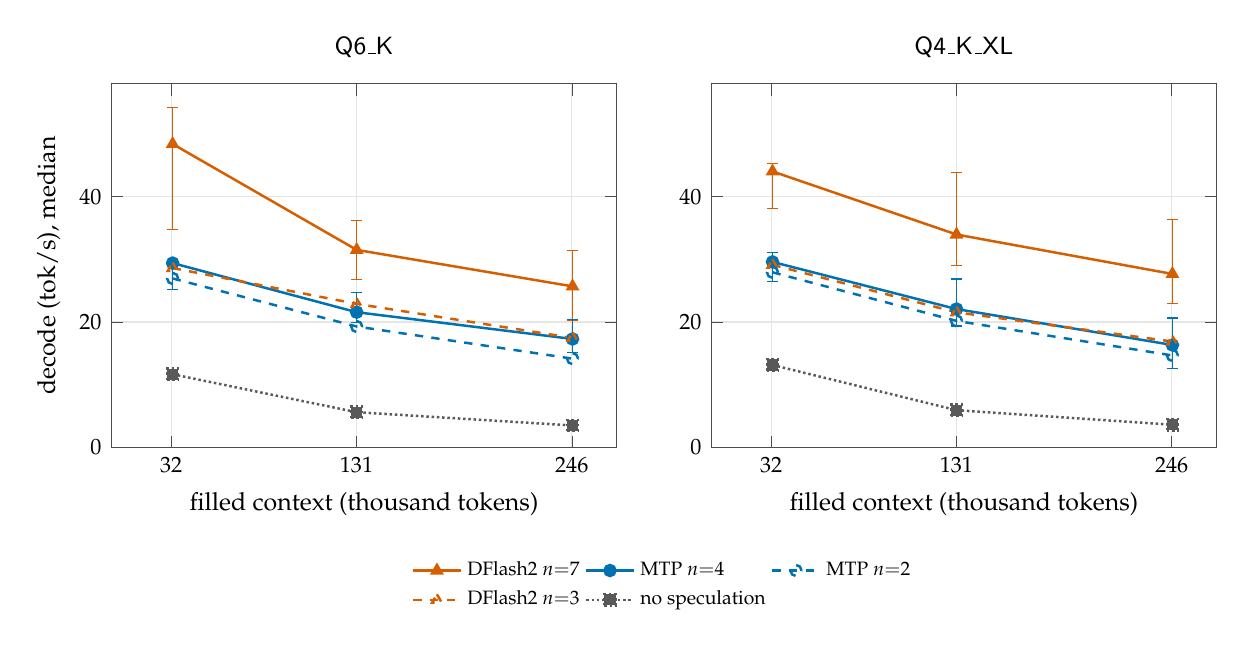
\begin{tikzpicture}
\begin{groupplot}[group style={group size=2 by 1,horizontal sep=1.2cm,ylabels at=edge left},
  paper,width=8.0cm,height=6.2cm,
  xlabel={filled context (thousand tokens)},ylabel={decode (tok/s), median},
  xmin=0,xmax=270,ymin=0,ymax=58,xtick={32,131,246},
  legend style={font=\scriptsize}]
\nextgroupplot[title={\small\Qsix},legend to name=speclegend,legend columns=3,
  error bars/y dir=both,error bars/y explicit,error bars/error bar style={line width=0.5pt}]
\addplot[cbred,mark=triangle*] coordinates {(32.768,48.39) += (0,5.8) -= (0,13.7) (131.072,31.50) += (0,4.7) -= (0,4.7) (246.415,25.68) += (0,5.7) -= (0,5.4)};
\addplot[cbblue,mark=*] coordinates {(32.768,29.39) += (0,0.3) -= (0,4.2) (131.072,21.56) += (0,3.1) -= (0,1.7) (246.415,17.29) += (0,3.1) -= (0,2.1)};
\addplot[cbblue,mark=o,dashed] coordinates {(32.768,26.94) (131.072,19.28) (246.415,14.15)};
\addplot[cbred,mark=triangle,dashed] coordinates {(32.768,28.60) (131.072,22.89) (246.415,17.46)};
\addplot[black!65,mark=square*,densely dotted] coordinates {(32.768,11.66) (131.072,5.61) (246.415,3.49)};
\legend{DFlash2 $n{=}7$,MTP $n{=}4$,MTP $n{=}2$,DFlash2 $n{=}3$,no speculation}
\nextgroupplot[title={\small\Qfour},
  error bars/y dir=both,error bars/y explicit,error bars/error bar style={line width=0.5pt}]
\addplot[cbred,mark=triangle*] coordinates {(32.768,44.01) += (0,1.3) -= (0,5.9) (131.072,33.95) += (0,9.9) -= (0,5.0) (246.415,27.66) += (0,8.7) -= (0,4.7)};
\addplot[cbblue,mark=*] coordinates {(32.768,29.58) += (0,1.5) -= (0,3.1) (131.072,22.06) += (0,4.8) -= (0,2.7) (246.415,16.33) += (0,4.3) -= (0,3.8)};
\addplot[cbblue,mark=o,dashed] coordinates {(32.768,27.92) (131.072,20.17) (246.415,14.66)};
\addplot[cbred,mark=triangle,dashed] coordinates {(32.768,29.11) (131.072,21.54) (246.415,16.88)};
\addplot[black!65,mark=square*,densely dotted] coordinates {(32.768,13.14) (131.072,5.93) (246.415,3.61)};
\end{groupplot}
\node at ($(group c1r1.south)!0.5!(group c2r1.south)+(0,-1.75cm)$) {\pgfplotslegendfromname{speclegend}};
\end{tikzpicture}\\[8pt]
{\sffamily\scriptsize Greedy decoding, identical code prompts, q4\_0 KV cache, 1,024-token continuations (8 per point, 4 at 32K). Markers: median; bars: full range.\\[1pt]
Source: ``What Benchmarks Miss'' (L.\,H.\ Sim\~oes, 2026), Figure 7. Technical report, not peer reviewed. github.com/henrique-simoes/llm-quantization-damage}
\end{minipage}
\end{document}
